
%%
%% This is file `sample-manuscript.tex',
%% generated with the docstrip utility.
%%
%% The original source files were:
%%
%% samples.dtx  (with options: `manuscript')
%% 
%% IMPORTANT NOTICE:
%% 
%% For the copyright see the source file.
%% 
%% Any modified versions of this file must be renamed
%% with new filenames distinct from sample-manuscript.tex.
%% 
%% For distribution of the original source see the terms
%% for copying and modification in the file samples.dtx.
%% 
%% This generated file may be distributed as long as the
%% original source files, as listed above, are part of the
%% same distribution. (The sources need not necessarily be
%% in the same archive or directory.)
%%
%% The first command in your LaTeX source must be the \documentclass command.
\documentclass[manuscript,screen,review]{acmart}


\usepackage[main = greek, english]{babel} % For Greek language
\newcommand{\img}[1]
{
    \begin{center}
        \fcolorbox{black}{white}{\includegraphics[height=20em]{#1}}
    \end{center}

}
\usepackage{hyperref}
\usepackage{listings}
\usepackage{graphicx}
\usepackage{float}

% Helper Macros

\newcommand{\en}[1]{\foreignlanguage{english}{#1}}
\newcommand{\src}[1]{{\tt\en{#1}}}

%%
%% End of file `acmart.

\newcommand{\question}[1] % This is what you will use to create a new question
{
\par\noindent % Creates a new unindented paragraph
\phantomsection % Needed for hyperref compatibility with the \addcontensline command
\todo[inline, color=YellowOrange]{\textbf{#1}} % Uses the todonotes package to create a fancy box to put the question
\vspace{1em} % White space after the question before the start of the answer
}


%%
%% \BibTeX command to typeset BibTeX logo in the docs
\AtBeginDocument{%
  \providecommand\BibTeX{{%
    \normalfont B\kern-0.5em{\scshape i\kern-0.25em b}\kern-0.8em\TeX}}}

%% Rights management information.  This information is sent to you
%% when you complete the rights form.  These commands have SAMPLE
%% values in them; it is your responsibility as an author to replace
%% the commands and values with those provided to you when you
%% complete the rights form.
\setcopyright{}
\copyrightyear{2022}
\acmYear{}
\acmDOI{}

%% These commands are for a PROCEEDINGS abstract or paper.
\acmConference[]{}{}{}
\acmPrice{15.00}
\acmISBN{978-1-4503-XXXX-X/18/06}


%%
%% Submission ID.
%% Use this when submitting an article to a sponsored event. You'll
%% receive a unique submission ID from the organizers
%% of the event, and this ID should be used as the parameter to this command.
%%\acmSubmissionID{123-A56-BU3}

%%
%% The majority of ACM publications use numbered citations and
%% references.  The command \citestyle{authoryear} switches to the
%% "author year" style.
%%
%% If you are preparing content for an event
%% sponsored by ACM SIGGRAPH, you must use the "author year" style of
%% citations and references.
%% Uncommenting
%% the next command will enable that style.
%%\citestyle{acmauthoryear}

%%
%% end of the preamble, start of the body of the document source.
\begin{document}

%%
%% The "title" command has an optional parameter,
%% allowing the author to define a "short title" to be used in page headers.
\title{Εφαρμογή Εθελοντικού Οργανισμού \\ Εργασία στο μάθημα Βάσεις Δεδομένων - Ακαδημαϊκό Έτος: 2021-22}

%%
%% The "author" command and its associated commands are used to define
%% the authors and their affiliations.
%% Of note is the shared affiliation of the first two authors, and the
%% "authornote" and "authornotemark" commands
%% used to denote shared contribution to the research.



%%
%% By default, the full list of authors will be used in the page
%% headers. Often, this list is too long, and will overlap
%% other information printed in the page headers. This command allows
%% the author to define a more concise list
%% of authors' names for this purpose.

\author{Ι. Γεμου (1070525), Ε. Λάμπρου (1066519)}

\authornote{Η εργασία είναι προϊόν ισάξιας συνεισφοράς των δύο συγγραφέων.}
\email{}
\affiliation{%
  \institution{Tμήμα Ηλεκτρολόγων Μηχανικών και Τεχνολογίας Υπολογιστών}
 % \streetaddress{}
  %\city{ }
 % \state{}
  %\country{}
  %\postcode{}
}


%%
%% The abstract is a short summary of the work to be presented in the
%% article.
\begin{abstract}
Στο πλαίσιο του μαθήματος Βάσεις Δεδομένων μας ζητήθηκε να υλοποιήσουμε μια εφαρμογή εθελοντικού οργανισμού με βασικό στόχο την ανάδειξη των γνώσεων που αποκομίσαμε από το μάθημα και την εξοικείωσή μας το αντικείμενο. Ο ορισμός του μικρόκοσμου του συγκεκριμένου προβλήματος αφέθηκε στην δική μας κρίση, έτσι ώστε να είναι δική μας απόφαση το τι θα συμπεριλάμβουμε στην βάση δεδομένων μας. Η συγκεκριμένη εργασία  περιλαμβάνει τον σχεδιασμό της βάσης μέσω διαγράμματος
Οντοτήτων - Συσχετίσεων, καθώς και την πρακτική υλοποίηση μιας ιστοσελίδας μέσω της οποίας μπορούμε να αλληλεπιδράσουμε και να την χειριστούμε. Μέσα από αυτή τη διαδικασία εφαρμόσαμε γνώσεις που παρουσιάστηκαν θεωρητικά στο μάθημα, εξασκήσαμε
τεχνικές τις οποίες μάθαμε στο εργαστήριο και ήρθαμε αντιμέτωποι με νέα προβλήματα.
\end{abstract}

%%
%% The code below is generated by the tool at http://dl.acm.org/ccs.cfm.
%% Please copy and paste the code instead of the example below.
%%


%%
%% Keywords. The author(s) should pick words that accurately describe
%% the work being presented. Separate the keywords with commas.
\keywords{βάσεις δεδομένων, σχεδιασμός μιας βάσης, διάγραμμα οντοτήτων-συσχετίσεων, σχεσιακό σχήμα, επικοινωνία με την βάση, \en{SQL}}

%%
%% This command processes the author and affiliation and title
%% information and builds the first part of the formatted document.
\maketitle

\section{Eισαγωγή}

Οι βάσεις δεδομένων χρησιμοποιούνται σήμερα εκτενώς για την αποθήκευση και διαχείριση μεγάλου όγκου δεδομένων. Είναι, λοιπόν, αναμενόμενο ένας εθελοντικός οργανισμός να χρειάζεται μία βάση δεδομένων για την κάλυψη των αναγκών του, αλλά και ένα \en{interface} για να αλληλεπιδρούν τα μέλη του μαζί της.

\section{Περιγραφή τησ Εργασίασ}

\subsection{Θέμα της εργασίας}
Θέμα της εργασίας μας είναι η ανάπτυξη μιας εφαρμογής εθελοντικού οργανισμού. Η προσέγγισή μας έχει σκοπό την οργάνωση των πληροφοριών που αφορούν τους εθελοντές, αλλά και την οργάνωση διαφόρων \en{events} και την διαχείριση των οικονομικών του οργανισμού. Θεωρήσαμε πως αυτά είναι τα πιο σημαντικά τμήματα που θα έπρεπε να εστιάσουμε.

\subsection{Βήματα που ακολουθήσαμε}
Κατά διάρκεια του εξαμήνου έγινε εκτενής ανάλυση της θεωρίας των βάσεων δεδομένων
ξεκινώντας από μια αφηρημένη μορφή, υλοποιώντας το διάγραμμα Οντοτήτων-Συσχετίσεων (\en{Entity - Relationship Diagram}) για τον μικρόκοσμό μας, το οποίο ορίζει τις οντότητες της βάσης μας, καθώς και τα γνωρίσματα που τις περιγράφουν και τις συσχετίσεις που τις συνδέουν.
Επόμενο βήμα ήταν η ανάπτυξη του σχεσιακού σχήματος (\en{Relational Schema}), στο οποίο μεταφερόμαστε από το αφηρημένο διάγραμμα οντοτήτων σε μία σαφέστερη και αυστηρότερα ορισμένη δομή.
\newpage
Έπειτα, ακολουθεί το προγραμματιστικό τμήμα του \en{project} μας:

\begin{itemize}
    \item Δημιουργία της βάσης δεδομένων
    \item Εισαγωγή δεδομένων στην βάση μας
    \item Κατασκευή ενός \en{website} για την επικοινωνία του χρήστη με την βάση μας
\end{itemize}
 Να σημειωθεί ότι χρησιμοποιήθηκε \en{SQLite}, αφού είναι ένα πιο \en{lightweight database management system}, γρήγορο στο να διαβάζει και να γράφει δεδομένα, υποστηρίζεται από την βασική βιβλιοθήκη της \en{Python}, είναι συμβατό με όλα τα λειτουργικά συστήματα και γλώσσες προγραμματισμού, δωρεάν και \en{open source}!

\subsection{Περιγραφή του Μικρόκοσμου}
Ο μικρόκοσμός μας θα μπορούσε να διαχωριστεί σε τρείς υποκατηγορίες οι οποίες περιληπτικά είναι:
\begin{itemize}
    \item Διαχείριση των εθελοντών και των μελών:\\
    Θεωρήσαμε πώς όταν κάποιος μπαίνει στο \en{website} μας θα είναι ένα απλό μέλος. Προφανώς ένας εθελοντής ή ένας εργαζόμενος του οργανισμού είναι επίσης μέλη, τα οποία έχουν αρμοδιότητες.
    \item Οργάνωση δράσεων:\\
    Οι εθελοντές και οι εργαζόμενοι είναι αυτοί που δουλεύουν για την πραγματοποίηση των \en{events}.
    \item Διαχείριση των οικονομικών (είσοδα και έξοδα):\\
    Διάφοροι εργαζόμενοι μπορούν να διαχειρίζονται τα οικονομικά του οργανισμού.
\end{itemize}

\subsection{Tο διάγραμμα Οντοτήτων-Συσχετίσεων}

Όπως αναφέρθηκε προγουμένως, το πρώτο βήμα για τον σχεδιασμό της βάσης μας ήταν η δημιουργία του \en{Entity-Relationships Diagram}, το οποίο απεικονίζει τις βασικές οντότητές μας, τα γνωρίσματά τους και τις διασυνδέσεις των οντοτήτων μεταξύ τους.


Στην παρακάτω εικόνα φαίνεται ο σχεδιασμός μας:
\img{./images/erd.png}
Αναλυτικότερα:

Στο αριστερό μέρος του διαγράμματος παρατηρούμε πως ένας εθελοντικός οργανισμός αρχικά αποτελείται από διάφορα μέλη. Ένα άτομο, μπορεί να είναι είτε απλός \en{member}, αλλά εκτός από αυτό μπορεί να είναι επιπλέον και \en{volunteer} και \en{employee} ή και τα δύο. Μπορεί να παρατηρήσει κανείς πώς επιλέξαμε η οντότητα \en{Member} να είναι \en{Superclass} των δύο  \en{overlapping} οντοτήτων \en{Volunteer} και \en{Employee}. Σχεδιάστηκε οι δύο οντότητές μας να είναι \en{overlapping}, διότι θεωρήσαμε ότι ένα μέλος μπορεί να είναι ταυτόχρονα και εθελοντής και εργαζόμενος. Επίσης αποφασίσαμε να έχουν \en{Partial Specialization} γιατί δεν είναι απαραίτητο ένας \en{Member} να είναι είτε \en{Volunteer } ή \en{Employee}.

Οι εθελοντές του οργανισμού ανήκουν σε ομάδες, τις οποίες διαχειρίζεται και οργανώνει κάποιος εργαζόμενος. Επίσης οι εθελοντές δουλεύουν σε \en{tasks} τα οποία δημιουργεί ένας εργαζόμενος.
Προφανώς, ένα \en{tasks} σχετίζεται με τουλάχιστον ένα \en{Event}. Κάθε \en{Event} ανήκει σε μία ευρύτερη κατηγορία (\en{Event Category}).

Παρατηρούμε πως ένα μέλος μπορεί να συμμετέχει σε \en{Events}, και η συμμετοχή του αυτή μπορεί να οδηγήσει σε πιθανό εισόδημα για τον οργανισμό. Βλέπουμε ότι η οντότητα \en{Income} είναι \en{Superclass} των \en{disjoint} οντοτήτων \en{Sale, Service, Donation} και έχουμε \en{totally specialization} σε μία από τις τρεις. Αυτό σημαίνει πως ένα \en{income} θα είναι υποχρεωτικά είτε \en{service} είτε \en{sale} ή \en{donation}.

Ακόμη, ένα \en{Event} εκτός από τα έσοδα που μπορεί να συγκεντρώσει, ίσως να απαιτεί και κάποια έξοδα. Βλέπουμε ότι ένα έσοδο σχετίζεται με μηδέν ή περισσότερα έξοδα και ότι ένα έξοδο αντιστοιχεί σε ένα ακριβώς έσοδο.

\subsection{Το Σχεσιακό Σχήμα}

Το αμέσως επόμενο βήμα για τη σχεδίαση της βάσης δεδομένων μας ήταν η μεταφορά
από το διάγραμμα οντοτήτων συσχετίσεων στο σχεσιακό σχήμα. Το χαρακτηριστικό
αυτής της διαδικασίας είναι πως οι οντότητες και σχέσεις του \en{ERD}
μετατρέπονται σε πίνακες που περιέχουν τα κατάλληλα γνωρίσματα.

Πιο συγκεκριμένα, χρησιμοποιήσαμε το εργαλείο \en{ERDPlus} και δημιουργήσαμε τους πίνακες, ορίζοντας τους τύπους δεδομένων, αποφασίζοντας ποια από αυτά θα είναι πρωτεύοντα κλειδιά και ποια 
ξένα κλειδιά που θα αναφέρονται σε άλλους πίνακες, υποστηρίζοντας έτσι την επικοινωνία μεταξύ των πινάκων της βάσης μας. 

Στην παρακάτω εικόνα φαίνεται ο σχεδιασμός μας:

\img{./images/schema.png}


\section{Η Εφαρμογή}
Είναι προφανές ότι η επικοινωνία με την βάση μας πρέπει να πλαισιώνεται μέσω μιας εφαρμογής. Στην συγκεκριμένη περίπτωση αποφασίσαμε να κατασκευάσουμε ένα \en{Website} το οποίο να τρέχει στο \en{localhost}. Για την δημιουργία του \en{site} μας αποφασίσαμε να κάνουμε χρήση του \en{Django Framework} της \en{Python}, το οποίο μπορεί γενικά να χρησιμοποιηθεί τόσο για \en{backend} όσο και για \en{frontend}. 

Στην εργασία μας χρησιμοποιούμε το \en{Django} μόνο για το \en{frontend}. Η δημιουργία των πινάκων της βάσης και η εισαγωγή των δεδομένων σε αυτή γίνεται με \en{raw SQL}.

Oι λόγοι που επιλέξαμε το συγκεκριμένο \en{framework} είναι διότι:
\begin{itemize}
    \item Επιβάλει συγκεκριμένη δόμηση του κώδικα με βάση το \en{Model View Template (MVT)}
    \item Διαθέτει επικοινωνία με \en{post request} μεταξύ \en{server} και \en{client}
    \item Περιλαμβάνει πλήρες και εύχρηστο σύστημα παραγωγής στατικού \en{HTML} κώδικα
    \item Έχει ένα σαφές και πλήρες \en{documentation}
\end{itemize}

\subsection{Δεδομένα}
Τα δεδομένα που φορτώθηκαν στην βάση μας δημιουργήθηκαν με την βοήθεια ενός \en{random generator} που κατασκευάστηκε στην \en{python}. Αυτός ο \en{generator} δημιουργεί τυχαία ονόματα μελών, ημερομηνίες, ονόματα \en{events}, ομάδων και \en{task} και τα χρηματικά ποσά των εισόδων και εξόδων.

\subsection{Περιγραφή}

Το \en{Website} αποτελείται από τις εξής βασικές σελίδες:
\begin{itemize}
    \item \en{Home}
    \item \en{Volunteer}
    \item \en{Management}
\end{itemize}

Όταν κάποιος εισέρχεται στην ιστοσελίδα μας βλέπει το \en{Home page}, όπου
μπορεί να βρει ποια \en{events} διαδραματίζονται αυτήν την περίοδο στον
εθελοντικό οργανισμό, αλλά και ένα αρχείο περασμένων \en{events}. Αυτή η σελίδα
είναι ορατή από όλους όσους την επισκέπτονται. 

Στο κάτω μέρος της σελίδας έχει προστεθεί ένα πεδίο \en{"Did you know"} στο
οποίο αναγράφονται κάποια \en{fun facts } για τον οργανισμό μας! 

Επίσης στην σελίδα υπάρχει ένα \en{button "Join Us"} που όταν κάποιος το
πατήσει μεταφέρεται σε μία σελίδα όπου μπορεί να κάνει σύνδεση με το
ονοματεπώνυμό του. Αφού συνδεθεί, μεταφέρεται αυτόματα στο \en{profile} του.

Επιπλέον στην αρχική μας σελίδα, υπάρχει το \en{button "Support Us"} (το οποίο
αν κάποιος δεν έχει κάνει \en{join}, ανακατευθύνεται στην σελίδα \en{Join Us}),
όπου μπορεί ο οποιοσδήποτε να προσφέρει ένα χρηματικό ποσό στον οργανισμό μας,
είτε μέσω μιας δωρεάς, είτε μέσω μιας αγοράς ή εμμέσως, προσφέροντας κάποιου
είδους υπηρεσία. Οι δωρεές, οι πωλήσεις και οι προσφορές υπηρεσιών αναφέρονται
σε κάποιο \en{Event}.

Όταν κάποιος πατήσει πάνω σε κάποιο \en{Event}, μπορεί να δει περισσότερες
πληροφορίες για αυτό, όπως ημερομηνίες διεξαγωγής, την κατηγορία στην οποία
ανήκει, τους συμμετέχοντες και τα \en{Task} που σχετίζονται με το \en{Event}. 

Πατώντας το \en{button "Participate"}, η σελίδα ανανεώνεται αυτόματα και μπoρεί
να δει το όνομά του στους συμμετέχοντες.

Αν τώρα κάνουμε κλικ σε ένα \en{Task} μεταφερόμαστε σε μία σελίδα όπου μπορούμε
να επιλέξουμε αν θέλουμε να συμμετάσχουμε στη διεξαγωγή του. Ώστοσο αυτό μπορεί
να γίνει μόνο εάν δεν είναι ήδη ολοκληρωμένο. Προφανώς, το άτομο που αποφασίζει
αν έχει ολοκληρωθεί το \en{task} είναι ο δημιουργός του. Τα ολοκληρωμένα
\en{tasks} τονίζονται με πράσινο χρώμα.

Για να μπορέσει όμως κάποιος να συμμετέχει στην διεκπεραίωση ενός \en{task}
πρέπει να είναι εθελοντής. Επομένως πρέπει να μεταφερθεί στην σελίδα
\en{Volunteer} και να κάνει κλικ στο \en{button "Become o Volunteer"}. Επιπλέον
στην σελίδα \en{Volunteer} είναι ορατές όλες οι ομάδες και όλα τα πρόσφατα
\en{tasks}. Αν κάποιος πατήσει πάνω στο όνομα μίας ομάδας θα κατευθυνθεί σε μία
σελίδα όπου περιέχονται πληροφορίες για την ομάδα ( μέλη, περιγραφή αλλά και
εργασίες του κάθε μέλους) και μπορεί είτε να γίνει μέλος της ή να φύγει από την
ομάδα (αν είναι μέλος της ήδη).

Πατώντας το όνομα ενός μέλους μπορεί κάποιος να δει ένα σύντομο \en{profile}
του, καθώς και τις ομάδες στις οποίες συμμετέχει και τις εργασίες που
απασχολείται.

Τέλος, υπάρχει η σελίδα \en{Management}, η οποία όμως δεν είναι ορατή από όλους
και περιλαμβάνει την οικονομική διαχείριση του οργανισμού. Η σελίδα αυτή είναι
ορατή από τους εργαζόμενους του εθελοντικού οργανισμού και περιλαμβάνει όλες
τις πρόσφατες συναλλαγές και τις αξίες των εισόδων και εξόδων. Επίσης, σε συτήν
την σελίδα μπορεί κάποιος εργαζόμενος να προσθέσει καινούργια έξοδα για τον
οργανισμό, να δημιουργήσει νέες ομάδες και εργασίες και κατηγορίες \en{event}. 

\subsection{\en{SQL Queries}}
Ένα σημαντικό τμήμα της εργασίας μας ήταν η διατύπωση ενδεικτικών \en{SQL Queries} για κάποιες αναζητήσεις στην βάση δεδομένων μας.

Για παράδειγμα:\\
\textbf{Πληροφορίες για μία ομάδα:}
    \selectlanguage{english}
    \begin{lstlisting}
    SELECT T.name, T.description, M.name as mgr_name, M.surname as mgr_surname, 
            (SELECT IIF(TM.end_date is NULL, M.id, NULL)) as mgr_id, 
            (
                SELECT name FROM 
                (
                    SELECT atm.name || ' ' || atm.surname as name, COUNT(task.id) as task_cnt 
                    FROM active_team_members as atm JOIN works_on ON atm.id = works_on.volunteer 
                    JOIN task ON works_on.task = task.id
                    WHERE 
                    atm.team_name = T.name and task.completed = true and
                    task.due_date > DATETIME('now', '-30 day')
                    GROUP BY atm.id ORDER BY task_cnt DESC
                )
            ) as best_volunteer
                    FROM team as T JOIN team_management as TM ON T.name = TM.team
                    LEFT JOIN member as M on M.id = TM.employee
                    WHERE T.name = team_name
                    ORDER BY TM.start_date DESC LIMIT 1)
    
    \end{lstlisting}
\selectlanguage{greek}
        
Στο συγκεκριμένο \en{query} βρίσκουμε επίσης τον καλύτερο εθελοντή μίας ομάδας για να τον εμφανίσουμε στις πληροφορίες της!\\

\newpage
\textbf{Πληροφορίες για το κάθε μέλος:}
    \selectlanguage{english}
    \begin{lstlisting}
    SELECT name, surname, join_date, 
        (
            SELECT COUNT(*) FROM works_on JOIN task on works_on.task = task.id
            WHERE volunteer = M.id AND task.completed = false
        )   AS tasks_working_on, 
        (
            SELECT COUNT(*) FROM works_on JOIN task on works_on.task = task.id
            WHERE volunteer = M.id AND task.completed = true
        )   AS tasks_completed,
        (
            SELECT category FROM 
            (
                SELECT E.category, COUNT(*) as event_cnt
                FROM volunteer_task_assigned as VTA, task as VT, event as E 
                WHERE VTA.volunteer_id = M.id AND
                VT.id = VTA.task_id AND E.id = VT.event 
                GROUP BY E.category ORDER BY event_cnt DESC LIMIT 1
            )
        )   AS favorite_event_category
        FROM member as M LEFT JOIN volunteer AS V USING(id)
        WHERE M.id = (volunteer_id)
    \end{lstlisting}
    \selectlanguage{greek}
    
    Στο συγκεκριμένο \en{query} βρίσκουμε την αγαπημένη κατηγορία \en{events} του κάθε μέλους!\\
\textbf{Τα μέλη τα οποία είναι \en{best buddies}, δηλαδή παρακολούθησαν τα περισσότερα \en{events} μαζί:}
    \selectlanguage{english}
    \begin{lstlisting}
    SELECT m1.name || ' ' || m1.surname as name1, m2.name || ' ' || m2.surname as name2, 
            (
                SELECT COUNT(*) FROM 
                (
                    SELECT event FROM event_participation WHERE member = m1.id
                    INTERSECT
                    SELECT event FROM event_participation WHERE member = m2.id
                )
            ) AS common
             FROM member as m1, member as m2 WHERE m1.id != m2.id
             ORDER BY common DESC LIMIT 1
    \end{lstlisting}
    \selectlanguage{greek}

\newpage
\textbf{Έσοδα ανά τρίμηνο:}
\selectlanguage{english}
    \begin{lstlisting}
      SELECT SUM(value) as total, strftime('%Y', date) AS year, strftime('%m', date) / 3 + 1
      as quarter
      FROM income GROUP BY year, 
      quarter ORDER BY year;
    \end{lstlisting}
\selectlanguage{greek}

\textbf{Η μεγαλύτερη δωρεά:}

    \selectlanguage{english}
    \begin{lstlisting}
    SELECT MAX(value) as value, member.name || ' ' || member.surname as name, income.date 
        FROM income join event_participation as p on income.participation = p.id
        join member on p.member = member.id
        WHERE income.id IN 
        (
            SELECT income FROM donation
        )
    \end{lstlisting}
    \selectlanguage{greek}

Ένα σημαντικό κομμάτι της εργασίας μας ήταν η ανάπτυξη μηχανισμών για την συγγραφή συντομότερου κώδικα, όπως αναφέρεται παρακάτω.

\subsection{\en{Views}}

Χρησιμοποιήσαμε \en{Views} έτσι ώστε να συντομεύουμε τον κώδικα μας σε περίπλοκα \en{SQL Queries}. Tα \en{Views} είναι εικονικοί πίνακες οι οποίοι μπορεί να περιέχουν δεδομένα από έναν ή περισσότερους πίνακες της βάσης μας. 

Για παράδειγμα:

    \selectlanguage{english}
    \begin{lstlisting}
        CREATE VIEW team_members(volunteer_id, name, surname, team_name) AS
        SELECT M.id, M.name, M.surname, TP.team
        FROM team_participation as TP, member as M
        WHERE TP.volunteer = M.id;
    \end{lstlisting}
    \selectlanguage{greek}

Το συγκεκριμένο \en{view} περιέχει τα μέλη μιας ομάδας ανεξαρτήτως αν είναι ενεργά ή όχι.

    \selectlanguage{english}
    \begin{lstlisting}
        CREATE VIEW active_team_members(name, surname, id, team_name) AS
        SELECT M.name, M.surname, M.id, T.name 
        FROM team_participation ΑS
        TP JOIN team as T ON TP.team = T.name JOIN member as M ON TP.volunteer = M.id 
        WHERE TP.end_date is NULL;
    \end{lstlisting}
    \selectlanguage{greek}

Παραπάνω δημιουργούμε έναν εικονικό πίνακα που περιέχει μόνο τα ενεργά μέλη μίας ομάδας.
    
    \selectlanguage{english}
    \begin{lstlisting}
        CREATE VIEW 
        volunteer_task_assigned(volunteer_id, volunteer_name, volunteer_surname, task_id, task_name) 
        AS
        SELECT M.id, M.name, M.surname, T.id, T.name
        FROM task as T, member as M, works_on as W
        WHERE W.task = T.id AND W.volunteer = M.id;
    \end{lstlisting}
    \selectlanguage{greek}
    
Στην συγκεκριμένη περίπτωση, αντλούμε όλα τα \en{tasks} στα οποία απασχολείται ένας εθελοντής.

    \selectlanguage{english}
    \begin{lstlisting}
        CREATE VIEW active_event(name, id) AS
        SELECT name, id FROM event WHERE event.end_date > date('now') 
        OR event.end_date is NULL;
    \end{lstlisting}
    \selectlanguage{greek}

Το συγκεκριμένο \en{view} μας επιτρέπει να κατηγοροποιήσουμε ένα \en{event} ως ενεργό.

\subsection{\en{Indexes}}
Επιπλέον συμπεριλάβαμε \en{Indexes}, μηχανισμούς που μας επιτρέπουν να ανακτήσουμε δεδομένα από την βάση μας πολύ γρήγορα. 
Η εντολή \src{CREATE UNIQUE INDEX} δημιουργεί έναν μοναδικό δείκτη στον πίνακά μας. Για παράδειγμα:

    \selectlanguage{english}
    \begin{lstlisting}
    CREATE UNIQUE INDEX team_name_index ON team(name)
    \end{lstlisting}
    \selectlanguage{greek}
Δηλαδή το όνομα μίας ομάδας είναι μοναδικό.

\subsection{\en{Triggers}}
Ένα \en{Trigger} είναι μία αποθηκευμένη διαδικασία στην βάση δεδομένων, η οποία ενεργοποείται όταν συμβαίνει ένα ειδικό συμβάν που εμείς έχουμε επιλέξει.

Όπως φαίνεται παρακάτω, έχει δημιουργηθεί ένα \en{trigger} για την περίπτωση που ένα μέλος θέλει να παρακολουθήσει ένα \en{event} το οποίο δεν είναι ενεργό, δηλαδή έχει πραγματοποιηθεί στο παρελθόν.

    \selectlanguage{english}
    \begin{lstlisting}
    CREATE TRIGGER correct_participation_date 
    BEFORE INSERT ON event_participation
    BEGIN 
        SELECT 
        CASE 
            WHEN NEW.event NOT IN (SELECT id FROM active_event) 
            THEN 
              RAISE (ABORT, 'No new participations allowed on this event. It is not active.')
        END;
    END;
    \end{lstlisting}
    \selectlanguage{greek}

Αντίστοιχα, με το παρακάτω \en{trigger} δεν επιτρέπουμε σε κάποιον να ξανασυμμετέχει σε μία ομάδα, προτού απεγραφεί από αυτήν.

    \selectlanguage{english}
    \begin{lstlisting}
    CREATE TRIGGER double_team_participation 
    BEFORE INSERT ON team_participation
    BEGIN 
        SElECT 
        CASE 
          WHEN EXISTS (SELECT id FROM team_participation as TP 
          WHERE TP.volunteer = NEW.volunteer AND 
          TP.team = NEW.team AND TP.end_date is NULL) 
          THEN 
          RAISE(ABORT, 'A volunteer cannot join the same team twice without leaving first.')
        END;
    END;   
    \end{lstlisting}
    \selectlanguage{greek}    
    


\section{Συμπεράσματα}
Μέσω της συγκεκριμένη εργασίας ήρθαμε σε επαφή με ένα νέο για έμας εργαλείο, τις βάσεις δεδομένων. Θεωρούμε πως ήταν πολύ διδακτική για εμάς, από άποψης τόσο γνώσεων όσο και συνεργασίας.  

\section{Αξιολόγηση τησ εργασίασ μασ}
Το τελικό μας αποτέλεσμα θεωρούμε πως αντικατοπτρίζει επακριβώς την δουλειά μας κατά την διάρκεια του εξαμήνου. Στόχος μας ήταν η εργασία μας να προσεγγίζει όσο το δυνατόν καλύτερα τις απαιτήσεις ενός εθελοντικού οργανισμού, γι' αυτό και δώσαμε πολύ έμφαση στο πως θα στήσουμε την βάση μας σε θεωρητικό επίπεδο. Τέλος, το \en{Website} μας υλοποιήθηκε με σκοπό να έχει την μέγιστη δυνατή ευχρηστία και να προσεγγίζει το πρόβλημά μας ρεαλιστικά. 

\section{Αξιολόγηση τησ συνεργασίασ μασ}
Η συνεργασία μας κύλησε ομαλά καθ' όλη την διάρκεια του εξαμήνου. Φροντίζαμε να αναλαμβάνουμε \en{tasks} τα οποία προχωρούσαν παράλληλα, έτσι ώστε αν υπήρχε κάποιο πρόβλημα σε κάποιο τμήμα της δουλειάς να μην παρεμποδιζόταν η συνέχεια του \en{project}. Θεωρούμε πως αυτή η τακτική συνέβαλε καθοριστικά στην ομαλή διεκπεραίωση της εργασίας μας.

\section{Χρονοδιάγραμμα δράσεων}

Η κατασκευή του \en{ERD} τοποθετείται χρονικά στις πρώτες εβδομάδες μετά την ανακοίνωση του θέματός μας, όπου συλλέξαμε πληροφορίες που μας οδήγησαν στην πρώιμη κατασκευή του. Μετά την ενδιάμεση παρουσίαση αντιληφθήκαμε ότι η πρώτη αυτή υλοποίηση ήταν πολύ σύνθετη, οπότε έπειτα από διορθώσεις καταλήξαμε στην τελική του μορφή.

H διαδικασία κατασκευής του \en{Schema} έγινε κατά την διάρκεια της εβδομάδας μετά την ενδιάμεση παρουσίαση, όπου μετά τις διορθώσεις που έγιναν στο \en{ERD} δημιουργήσαμε την πρώτη μορφή του. Ωστόσο, με το πέρας των εβδομάδων και καθώς δημιουργούσαμε τους πίνακες της βάσης μας, έγιναν αρκετές τροποποιήσεις μέχρι να πάρει την τελική του μορφή.

Η δημιουργία της εφαρμογής ξεκίνησε περίπου στις αρχές Δεκεμβρίου, όπου παράλληλα δημιουργήσαμε την βάση μας και φορτώσαμε δεδομένα σε αυτή και ξεκινήσαμε την κατασκευή της ιστοσελίδας.
Η εργασία άρχισε να παίρνει την τελική της μορφή στα τέλη Δεκεμβρίου. Ωστόσο οι βελτιώσεις συνεχίστηκαν μέχρι περίπου 10 Ιανουαρίου, αφού προσθέσαμε κάποιες λειτουργίες και βελτιώσαμε κάποιες άλλες.

Η συγγραφή της αναφοράς ξεκίνησε περίπου στις 7 Ιανουαρίου και τελείωσε στις 12
Ιανουαρίου. H δημιουργία της παρουσίασης έγινε στις 14 Ιανουαρίου.

\section{Βιβλιογραφία}
\begin{itemize}
    \item Για την μορφοποίηση της ιστοσελίδας (εμφάνιση \en{LaTex document}): 
    
    \en{\url{https://github.com/vincentdoerig/latex-css}}
    \item \en{SQLite }:
    
    \en{\url{https://stackoverflow.com/questions/15819186/sqlite-create-unique-pair-of-columns}}
    
    \en{\url{ https://www.sqlitetutorial.net}}
    
    \item \en{Django Documentation}:
    
    \en{\url{https://docs.djangoproject.com/en/4.0/}}
\end{itemize}

\newpage
\section{Παράρτημα}

\subsection{\en{Showcase} της εφαρμογής}
Παρακάτω φαίνονται κάποια στιγμιότυπα από το \en{Website} μας:

\begin{figure}[H]
    \centering
    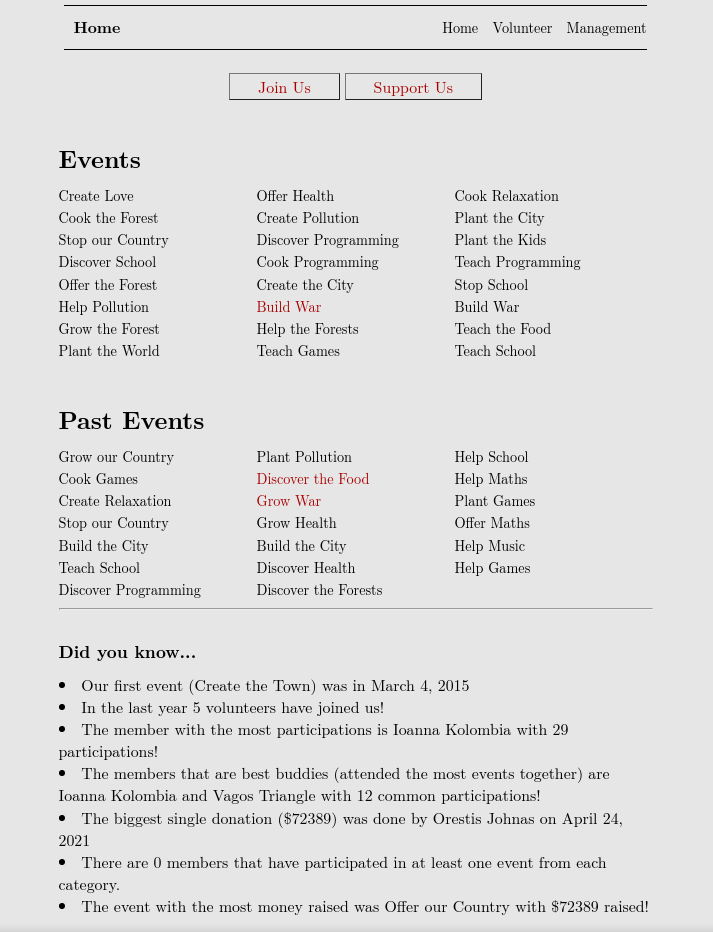
\includegraphics[width=.7\textwidth]{./images/homepage.png}
    \caption{H κύρια σελίδα μας}
\end{figure}

\begin{figure}[H]
    \centering
    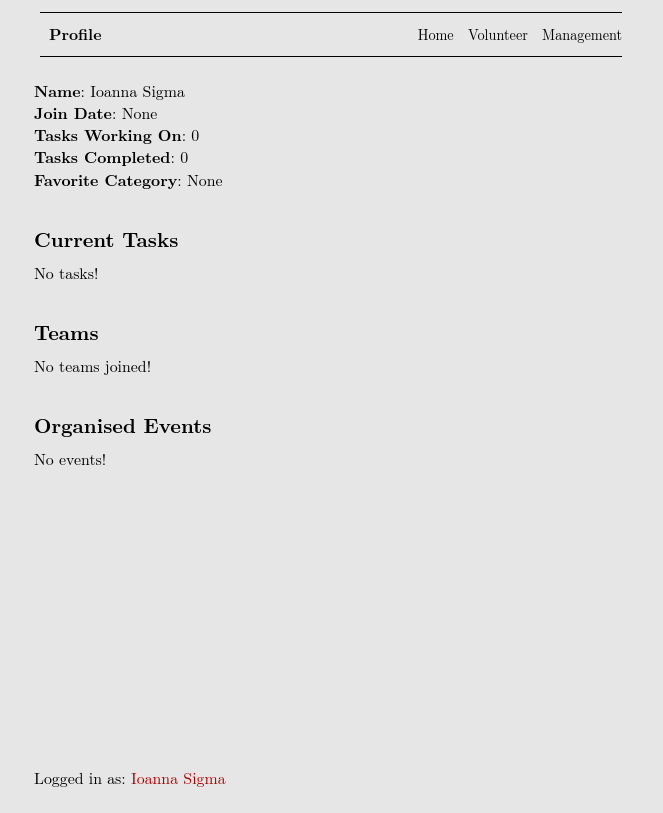
\includegraphics[width=.5\textwidth]{./images/profile.png}
    \caption{To προφίλ του χρήστη}
    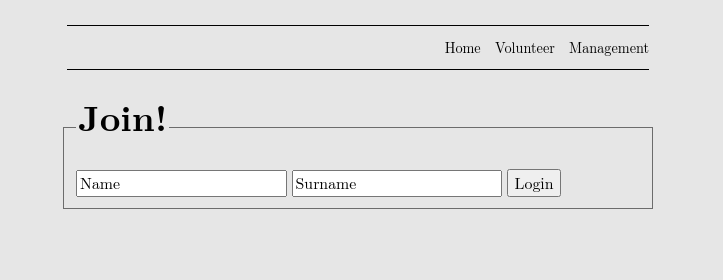
\includegraphics[width=.5\textwidth]{./images/join.png}
    \caption{Η σελίδα που μπορεί κάποιος να συνδεθεί και να έπειτα να δει το προφίλ του}
\end{figure}

\begin{figure}[H]
\centering
    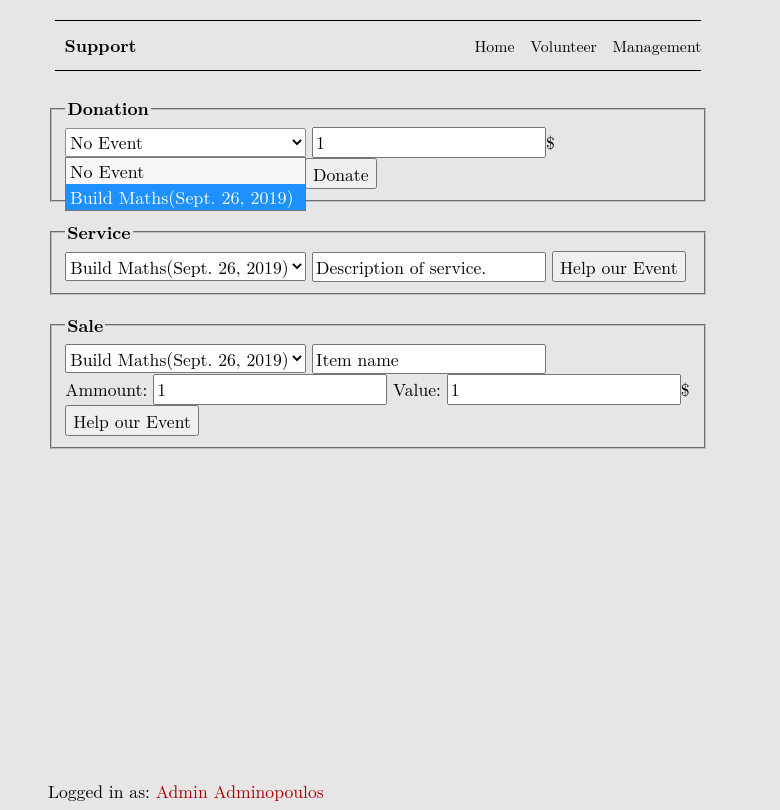
\includegraphics[width=.5\textwidth]{./images/support_example.png}
    \caption{Η σελίδα που μπορεί κάποιος να μας ενισχύσει}

    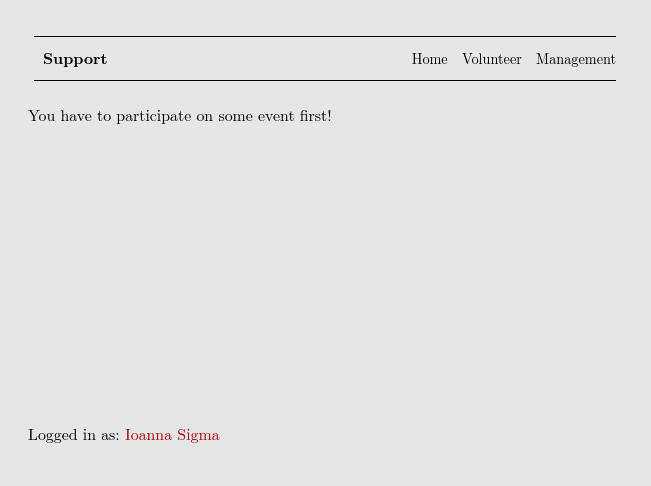
\includegraphics[width=.5\textwidth]{./images/support.png}
    \caption{Η σελίδα για κάποιον που δεν έχει παρακολουθήσει κάποιο \en{event}}
   
\end{figure}

\begin{figure}[H]
 \centering
 \centering
    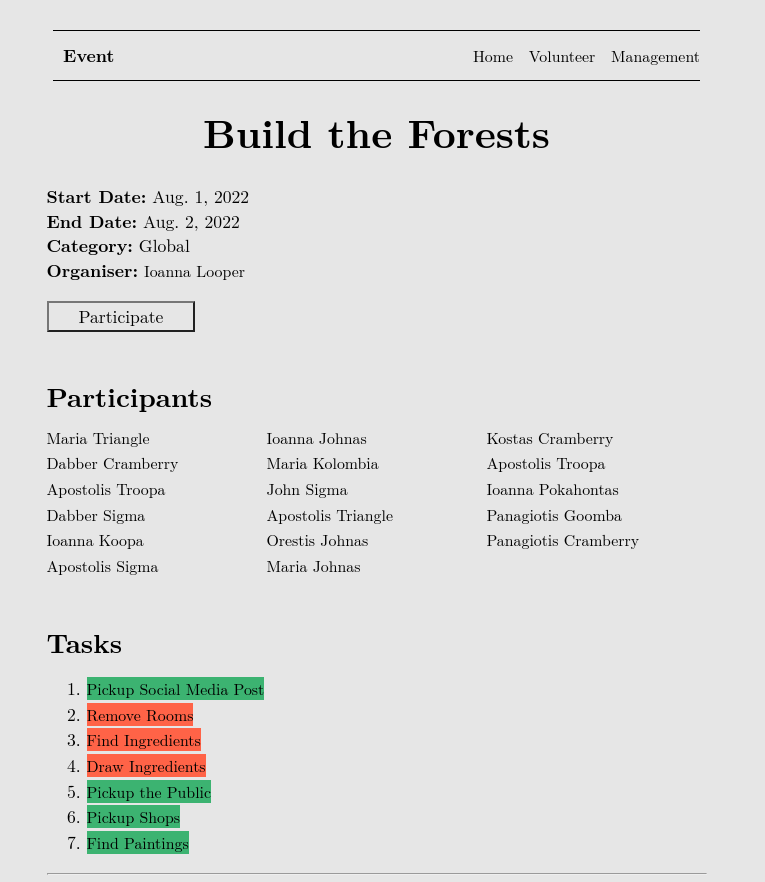
\includegraphics[width=.5\textwidth]{./images/eventparticipation.png}
    \caption{Ένα παράδειγμα ενός \en{event}, όπoυ κάποιος μπορεί να συμμετάσχει κάνοντας κλικ στο \en{Participate}}
    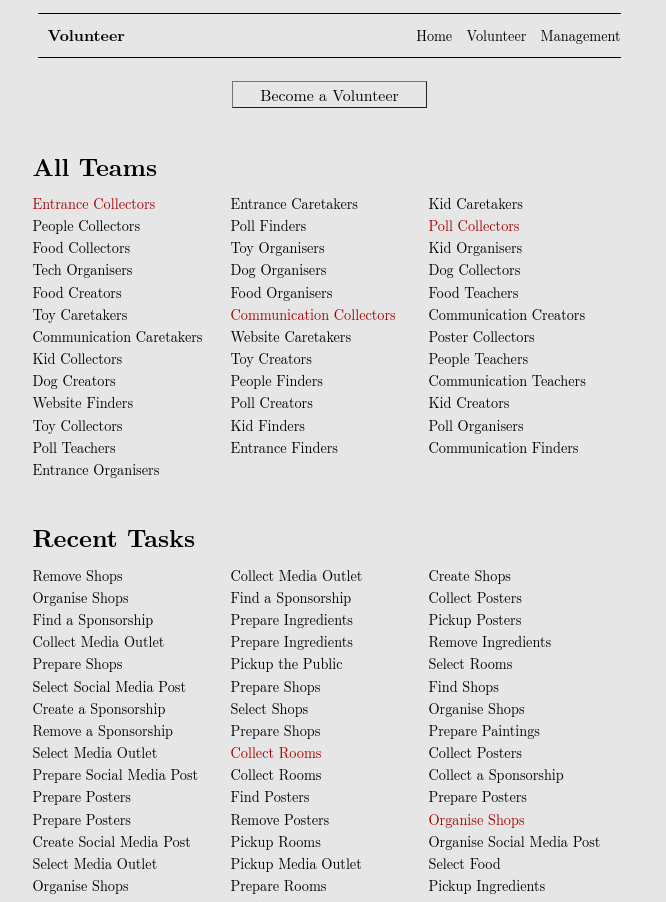
\includegraphics[width=.5\textwidth]{./images/volunteerpage.png}
    \caption{Οι σελίδα \en{volunteer}, όπυ είναι ορατές οι ομάδες και οι εργασίες}
\end{figure}

\begin{figure}[H]
 \centering
    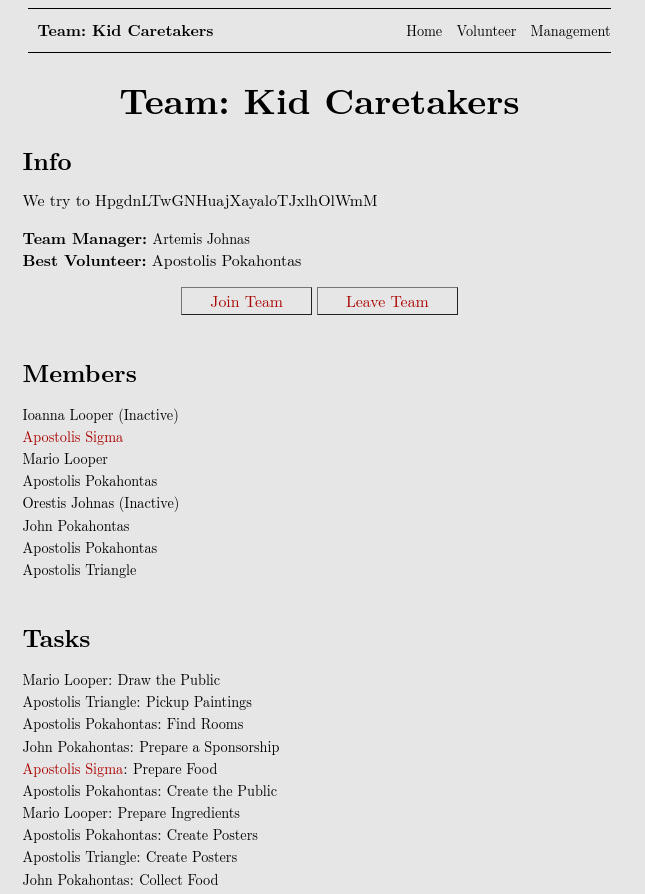
\includegraphics[width=.5\textwidth]{./images/teamExample.png}
    \caption{Παράδειγμα μίας ομάδας}
\centering
    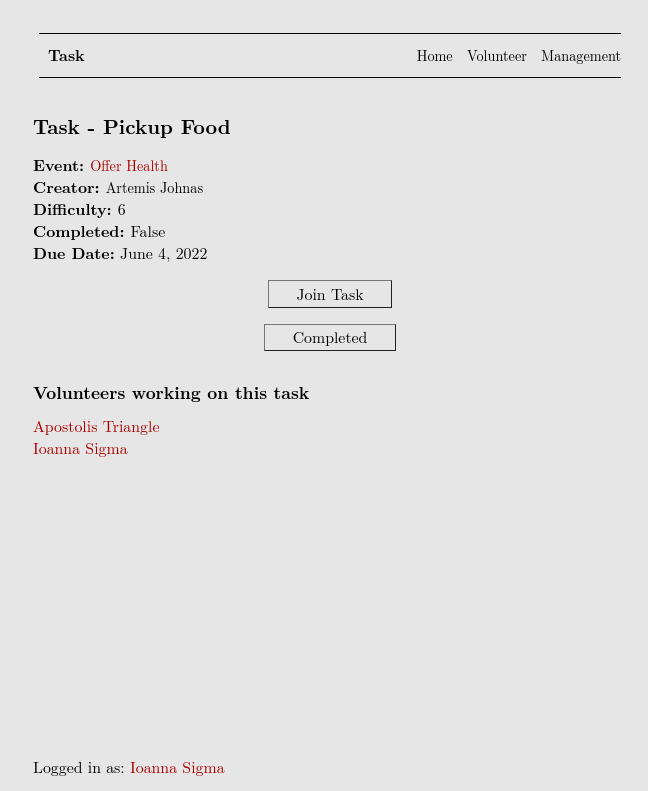
\includegraphics[width=.5\textwidth]{./images/joinTask.png}
    \caption{Μία εργασία όπου οι εθελοντές μπορούν να αναλάβουν }
   
\end{figure}

\begin{figure}[H]
\centering
 \centering
    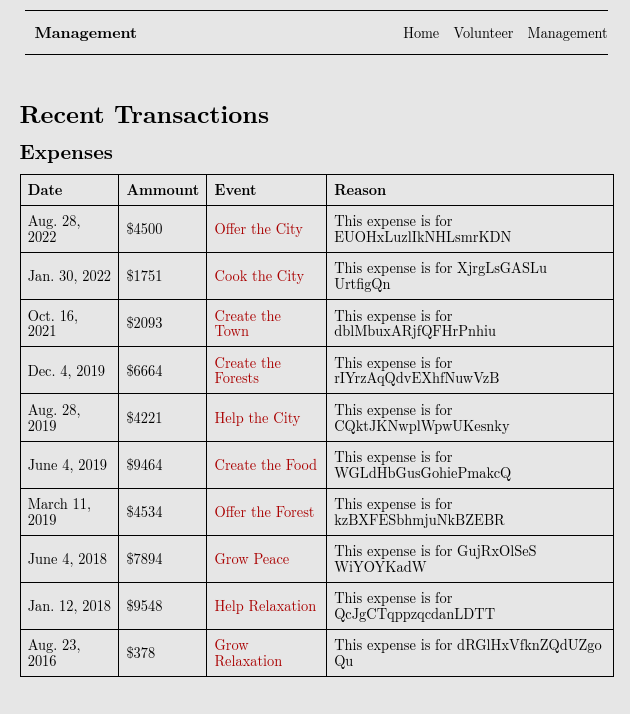
\includegraphics[width=.5\textwidth]{./images/expenses.png}
    \caption{Τα πρόσφατα έξοδα του οργανισμού}
    
    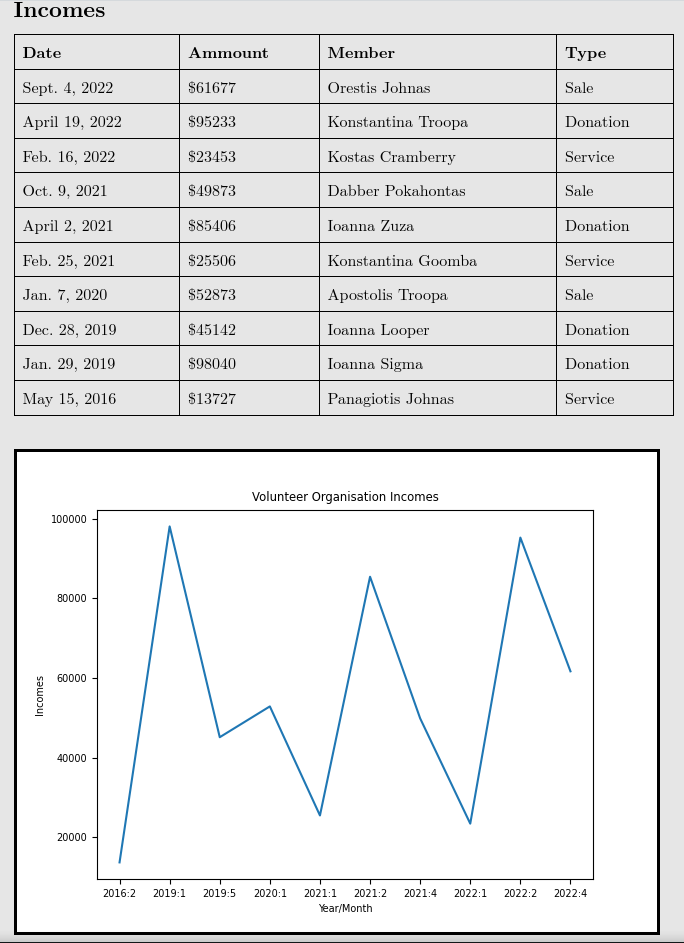
\includegraphics[width=.5\textwidth]{./images/incomes.png}
    \caption{Τα πρόσφατα έσοδα και διάγραμμα εσόδων}
  
\end{figure}

\begin{figure}[H]

    \centering
    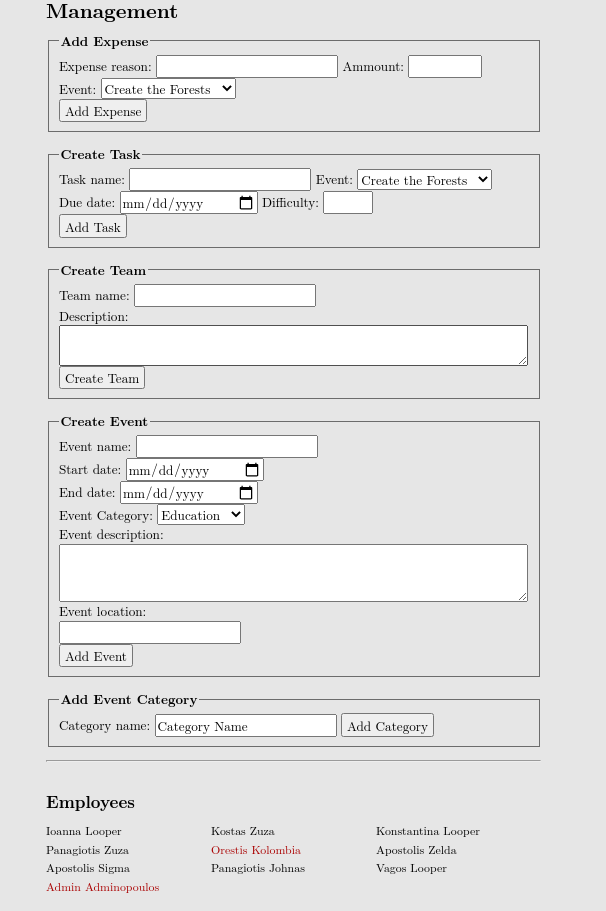
\includegraphics[width=.5\textwidth]{./images/management.png}
    \caption{H κατηγορία \en{Management} }
\end{figure}

\subsection{Σύνδεσμοι}
\en{Github Repository link}: \en{\url{https://github.com/Vagos/volunteer-organisation-app}}

\end{document}
\endinput
%%
%% End of file `sample-manuscript.tex'.
